\chapter{Medición de tiempos de ejecución}
Se ha mencionado en el capítulo anterior que el programa de extracción de puntos SIFT, $sift\_keypoints$, consta de dos partes principales entre otras como pueden ser cargar librerías, crear o modificar ficheros de texto o copiar información de una nube de puntos a otra. Estas dos partes son la extracción de vectores normales a la superficie descrita por la nube de puntos con la que trabaja el programa y la estimación de puntos SIFT.
\\
En este capítulo se va a presentar una forma sencilla de medir los tiempos de ejecución de estos dos procesos a la vez que se modifican los parámetros que influyen en ellos. De este modo, se determinará si será la estimación de normales o la de puntos SIFT la parte necesita ser llevada a hardware digital para su posterior optimización.

\section{Proceso de medición}
Trabajando en C++ como de costumbre, el proceso de medición de tiempos requiere la inclusión de la librería $ctime$ para lo cual se tiene al comienzo del código en $sift\_keypoints.cpp$:

\begin{lstlisting}[language=C++,breaklines]
	#include <ctime>
\end{lstlisting}

Incluída esta librería, ahora se pueden utilizar las variables globales $begin$,$end$ y $elapsed\_sec$ declaradas de la siguiente manera:

\begin{lstlisting}[language=C++,breaklines]
	clock_t begin,end;
	double elapsed_sec;
\end{lstlisting}

Las variables $begin$ y $end$ son del tipo $clock_t$ y sirven para almacenar cuentas de $clock\;\; ticks$ o ciclos de reloj mientras que $elapsed\_sec$ es del tipo double para almacenar el tiempo en segundos que ha llevado efectuar una determinada operación.\\
El proceso de medición de tiempo es el siguiente: 

\begin{lstlisting}[language=C++,breaklines]
	begin = clock();
	process();
	end = clock();
	
	elapsed_sec = double(end - begin)/CLOCKS_PER_SEC;
\end{lstlisting}

En primer lugar se almacena en $begin$ el valor devuelto por la función $clock()$, es decir, número de ciclos de reloj que han transcurrido en el procesador desde el inicio del programa hasta su llamada. A continuación se ejecuta el proceso cuyo tiempo de ejecución desea medirse, para este ejemplo, $process()$. Ahora se actúa de manera similar al primer paso ya que se almacena en $end$ el número de ciclos transcurridos desde el inicio del programa hasta la llamada a $clock()$ después de haberse ejecutado $process()$. Por último, se toma la diferencia de ciclos entre $end$ y $begin$ para saber cuántos ciclos ha tomado la ejecución de $process()$. Sin embargo esto no es una medida directa de tiempo por lo que el número de ciclos de ejecución del proceso se divide entre una constante, el número de ciclos que duran un segundo y que se llama $CLOCKS\_PER\_SEC$

Una vez visto cómo se mide el tiempo de ejecución de cualquier parte del programa $sift\_keypoints$, se rescata parte del código del mismo para indicar qué procesos van a ser sometidos a esta medición.
\\
En la parte de estimación de normales se analiza el método $compute$ el cual realiza todas las operaciones pertinentes para almacenar en $cloud\_normals$ los vectores normales a partir de $cloud\_xyz$:


\begin{lstlisting}[language=C++,breaklines]
  pcl::PointCloud<pcl::PointNormal>::Ptr cloud_normals (new 		pcl::PointCloud<pcl::PointNormal>);
  pcl::search::KdTree<pcl::PointXYZ>::Ptr tree_n(new pcl::search::KdTree<pcl::PointXYZ>());

  ne.setInputCloud(cloud_xyz);
  ne.setSearchMethod(tree_n);
  ne.setRadiusSearch(radius_search);
 
  std::cout << "Estimating normals in " << filename << " surface..." <<std::endl;

  begin = clock();
  ne.compute(*cloud_normals);
  end = clock();

  normal_estimation_time = double(end-begin)/CLOCKS_PER_SEC;
  std::cout << "Time needed for normal estimation (compute) in " << filename << ": " << normal_estimation_time << " seconds" << std::endl << std::endl;
\end{lstlisting}

Se procede de forma análoga en la parte de estimación de puntos SIFT puesto que, tras establecer el valor de los parámetros también se llama a un método $compute$ para efectuar la extracción de keypoints:

\begin{lstlisting}[language=C++,breaklines]
  pcl::SIFTKeypoint<pcl::PointNormal, pcl::PointWithScale> sift;
  pcl::PointCloud<pcl::PointWithScale>::Ptr result(new pcl::PointCloud<pcl::PointWithScale>);
  pcl::search::KdTree<pcl::PointNormal>::Ptr tree(new pcl::search::KdTree<pcl::PointNormal> ());
  sift.setSearchMethod(tree);
  sift.setScales(min_scale, n_octaves, n_scales_per_octave);
  sift.setMinimumContrast(min_contrast);
  sift.setInputCloud(cloud_normals);
 
  std::cout << "Estimating sift points in " << filename << "..." << std::endl;

  begin = clock();
  sift.compute(*result);
  end = clock();
  sift_estimation_time = double(end-begin)/CLOCKS_PER_SEC;
  std::cout << "Time needed for sift point extraction: " << sift_estimation_time << " seconds" << std::endl << std::endl;
\end{lstlisting}

Los tiempos de ejecución del método $compute$ se almacenan en $normal\_estimation\_time$ y $sift\_estimation\_time$ para la parte de estimación de normales y puntos SIFT, respectivamente.
\\
Para aportar mayor amplitud a los resultados obtenidos, se van a realizar mediciones de los métodos $compute$ variando ligeramente los parámetros involucrados en la estimación de normales y puntos SIFT. Como se ha visto en los fragmentos de código mostrados, la extracción de normales varía con un único parámetro, $radius\_search$, mientras que el tiempo de estimación de keypoints varía con $min\_scale$, $n\_octaves$ y $n\_scales\_per\_octave$. El parámetro $min\_contrast$ no afecta al tiempo del proceso estudiado porque, como se ha visto anteriormente, indica la dureza de la criba de los puntos SIFT ya obtenidos.

Las nubes sobre las que se han realizado las pruebas son las mismas que las mostradas en el capítulo anterior: $bunny.pc$, $cturtle.pcd$ y $milk\_cartoon\_all\_small\_clorox.pcd$

Tras efectuar la medición de tiempos junto a la variación de parámetros, éstos se han plasmado en diferentes gráficas. En primer lugar, se analizan los tiempos de estimación de normales y puntos SIFT variando el parámetro $radius\_search$ puesto que la extracción de normales es la primera operación y afecta a las que vienen después. El resultado se aprecia en las figuras 

\begin{figure}[!htb]
\minipage{0.32\textwidth}
  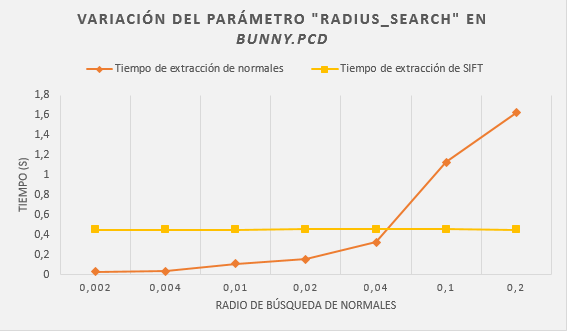
\includegraphics[width=\linewidth]{grafico_radius_bunny}
  \caption{Tiempos de estimación de normales y puntos SIFT en $bunny.pcd$ variando $radius\_search$.}\label{fig:grafico_radius_bunny}
\endminipage\hfill
\minipage{0.32\textwidth}
  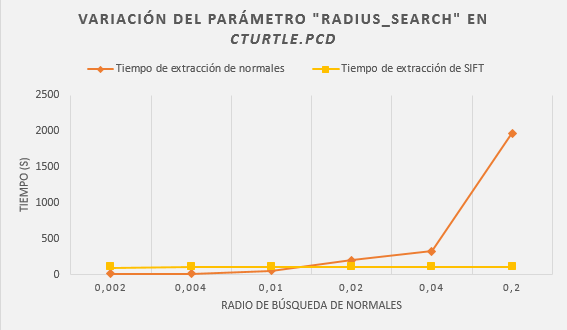
\includegraphics[width=\linewidth]{grafico_radius_cturtle}
  \caption{Tiempos de estimación de normales y puntos SIFT en $cturtle.pcd$ variando $radius\_search$.}\label{fig:grafico_radius_cturtle}
\endminipage\hfill
\minipage{0.33\textwidth}
  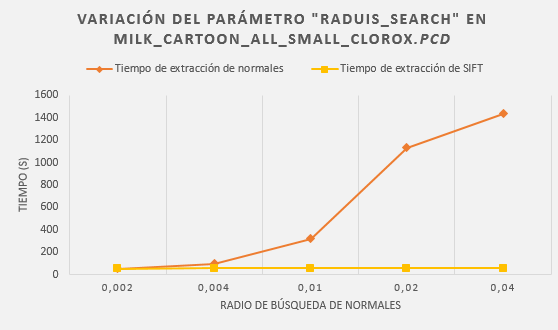
\includegraphics[width=\linewidth]{grafico_radius_milk}
  \caption{Tiempos de estimación de normales y puntos SIFT en $milk\_cartoon\_all\_small\_clorox.pcd$ variando $radius\_search$.}\label{fig:grafico_radius_milk}
\endminipage\hfill
\end{figure}


\section{Resultados}